%% This is an example first chapter.  You should put chapter/appendix that you
%% write into a separate file, and add a line \include{yourfilename} to
%% main.tex, where `yourfilename.tex' is the name of the chapter/appendix file.
%% You can process specific files by typing their names in at the 
%% \files=
%% prompt when you run the file main.tex through LaTeX.

\chapter{The Loop Gap Resonator}

As mentioned in the introduction, for many applied modalities within applications that use NV centers, the MW field (often denoted $B_1$ from NMR nomenclature), requires both high power and high uniformity to achieve high-fidelity quantum-state manipulation over the entire sample volume. As volumes are increased however, to maximize the number of NVs addressed without having a deleterious affect on the optimal measurement time, applying such a field becomes more difficult using standard approaches such as shorted coaxial loops \cite{clevenson2015broadband,chipaux2015magnetic}, microstrip waveguides \cite{andrich2017long,horowitz2012electron}, and 50 $\Omega$-terminated coaxial transmission lines \cite{li2010design,mrozek2015circularly,zhang2016microwave,zhang2018vector}. These broadband approaches allow arbitrary drive frequencies, however, the lack of resonant enhancement forces a compromise between the addressed volume and field strength. Section \ref{Planar} describes how planar lumped-element resonators such as split-ring resonators \cite{bayat2014efficient}, planar-ring resonators \cite{zhang2016microwave,sasaki2016broadband}, omega resonators \cite{twig2013ultra,horsley2018microwave,simpson2017electron}, and patch antennas \cite{zhang2016microwave} can improve coupling between the resonator and the NVs by resonantly enhancing the local $B_1$ field and thus enable MW driving over larger regions, but at the expense of bandwidth and thus, for an operational magnetometer, dynamic range. Additionally, planar resonators are shown to yield poor homogeneity in the planes normal to their surface and therefore lend themselves less to bulk magnetometry than to 2D imaging applications. To address this shortcoming 3D resonators and cavities can be employed such as enclosed metallic cavity resonators \cite{rose2017coherent}, enclosed dielectric resonators \cite{breeze2017continuous,floch2016towards,creedon2015strong}, open dielectric resonators \cite{kapitanova2017dielectric}, and three-dimensional lumped element resonators \cite{angerer2016collective}, which provide good field homogeneity and strong resonantly enhanced fields, but offer little to no optical access. Since all-optical initialization and readout is a primary benefit for many solid-state spin systems, including NV diamond \cite{doherty2013nitrogen}, such a trade-off is incompatible with many existing and envisioned applications \cite{schirhagl2014nitrogen}. 

To address this current shortcoming a three-dimensional tunable loop-gap resonator (LGR), based on the anode block of a cavity magnetron, is used to achieve desired MW drive strengths homogeneously over large areas. Additionally, its open geometry allows for good optical accessibility for interrogation volumes centered within the LGR cavity. Traditionally, the LGR has been used either as the anode block of cavity magnetrons \cite{}, or as a low frequency (2-4 GHz) lumped element resonator for electron paramagnetic resonance (EPR) studies \cite{}.  

\section{Resonant Enhancement of the MW field}

The LGR acts classically like an underdamped oscillator. It stores MWs within the confines of its geometrical structure by allowing the energy to oscillate back and forth between an electric and magnetic potential. At resonance ($\omega_0$) the ratio of magnetic energy to electric energy is 1. The time $\tau_ring$ the energy can oscillate before its power is reduced by a factor of 1/e is characterized by a dimensionless quantity called the Q-factor. It's defined by the following ratio
\begin{equation}
Q = \omega_0 \frac{Stored Energy}{Power Loss}.
\end{equation}
If the resonator is therefore continuously fed by an external power source an enhancement of the stored energy takes place that is proportional to both the current supplied and the Q-factor of the cavity. The magnitude of the magnetic flux within the center cavity (for a cylindrical resonator) is then given by
\begin{equation}
|B_1| \approx  \frac{\upmu_0}{2 r} \cdot I \cdot \sqrt{Q},
\end{equation}
where $\upmu_0$ is the vacuum permeability, $I$ is the supplied current, and $r$ is the cylinder radius. It's therefore clear that a resonant enhancement of the magnetic field amplitude is induced which is proportional to the square root of the Q-factor. 


\section{Model}

whatever

\subsection{Lumped element solutions} \label{circuit}

Theoretical framework for analyzing LGR for $m$ loops and $n$ gaps including field distribution calculations

\subsection{Field based solutions}

Theory giving solutions of LGR using bessel functions

\subsection{Coupling} \label{coupling}

Theory of coupling (mutual inductance, capcitance, etc)

\section{LGR Design}

Due to the loop gap resonator's existence since the early 20th century \cite{collins1948microwave} it has seen many variations and modifications all designed with particular applications in mind. Figure \ref{LGR_variation} shows the cross section of a variety of LGRs including rising-sun, vane, slot, and hole-and-slot type resonators. EPR experiments at low frequencies (2-4 GHz) quickly adopted the LGR as opposed to more traditional TE\textsubscript{102} type cavities because of the LGRs smaller size relative to the frequency of excitation. At 3 GHz the side length of the TE\textsubscript{102} cavity must be at least 5 cm which reduces drastically the cavity filling factor--a parameter necessary for the sensitivity of an EPR signal. Since many aspects of EPR spectroscopy are mirrored in NV magnetometry (requirement of homogeneous and strong microwave signals, frequency of operation, etc.) we selected to design a hole-and-slot type resonator found in many EPR applications \cite{}.  
\vspace{5mm}
\begin{figure}[h!]
\centering
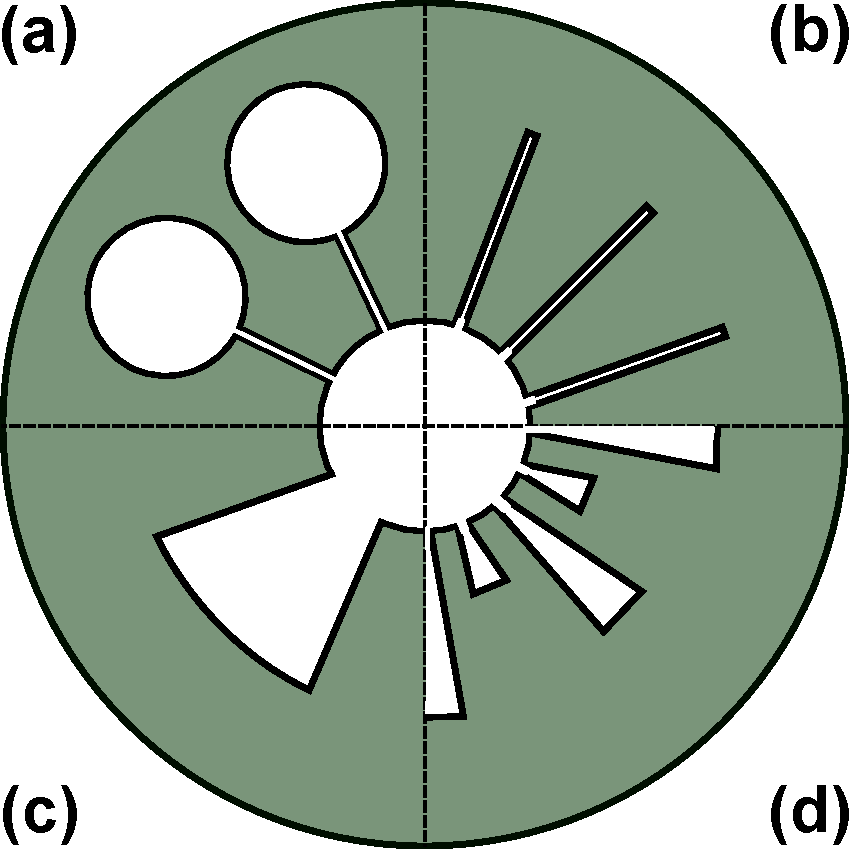
\includegraphics[scale = 0.5]{LGR_Variation.pdf}  
\caption{\textbf{Loop Gap Resonator Variations} \textbf{a)} Hole and Slot. \textbf{b)} Slot. \textbf{c)} Vane. \textbf{d)} Rising Sun - type}
\label{LGR_variation}
\end{figure}


\subsection{LGR}

A standard hole-and-slot LGR with $n$ outer loops can be approximated as $n$ coupled LC resonators oscillating in tandem at a target resonant frequency \cite{wood1984loop}. Circulating currents around the central and outer loops create a total inductance, as found in section \ref{circuit}, 

% When circuit model section is written take out these equations and simply reference them.

\begin{equation}
L \approx \frac{L_c n L_o}{n L_o + L_c},
\end{equation}\label{induct}

and charge at the gap walls create a total capacitance C, which is given by

\begin{equation}
C \approx \frac{\epsilon_r \epsilon_o A}{nd},
\end{equation} \label{cap}

which, when combined yield the resonant frequency

\begin{equation}
f_0 = \frac{1}{2 \pi \sqrt{LC}}.
\end{equation}

\begin{figure}[t!]
\centering
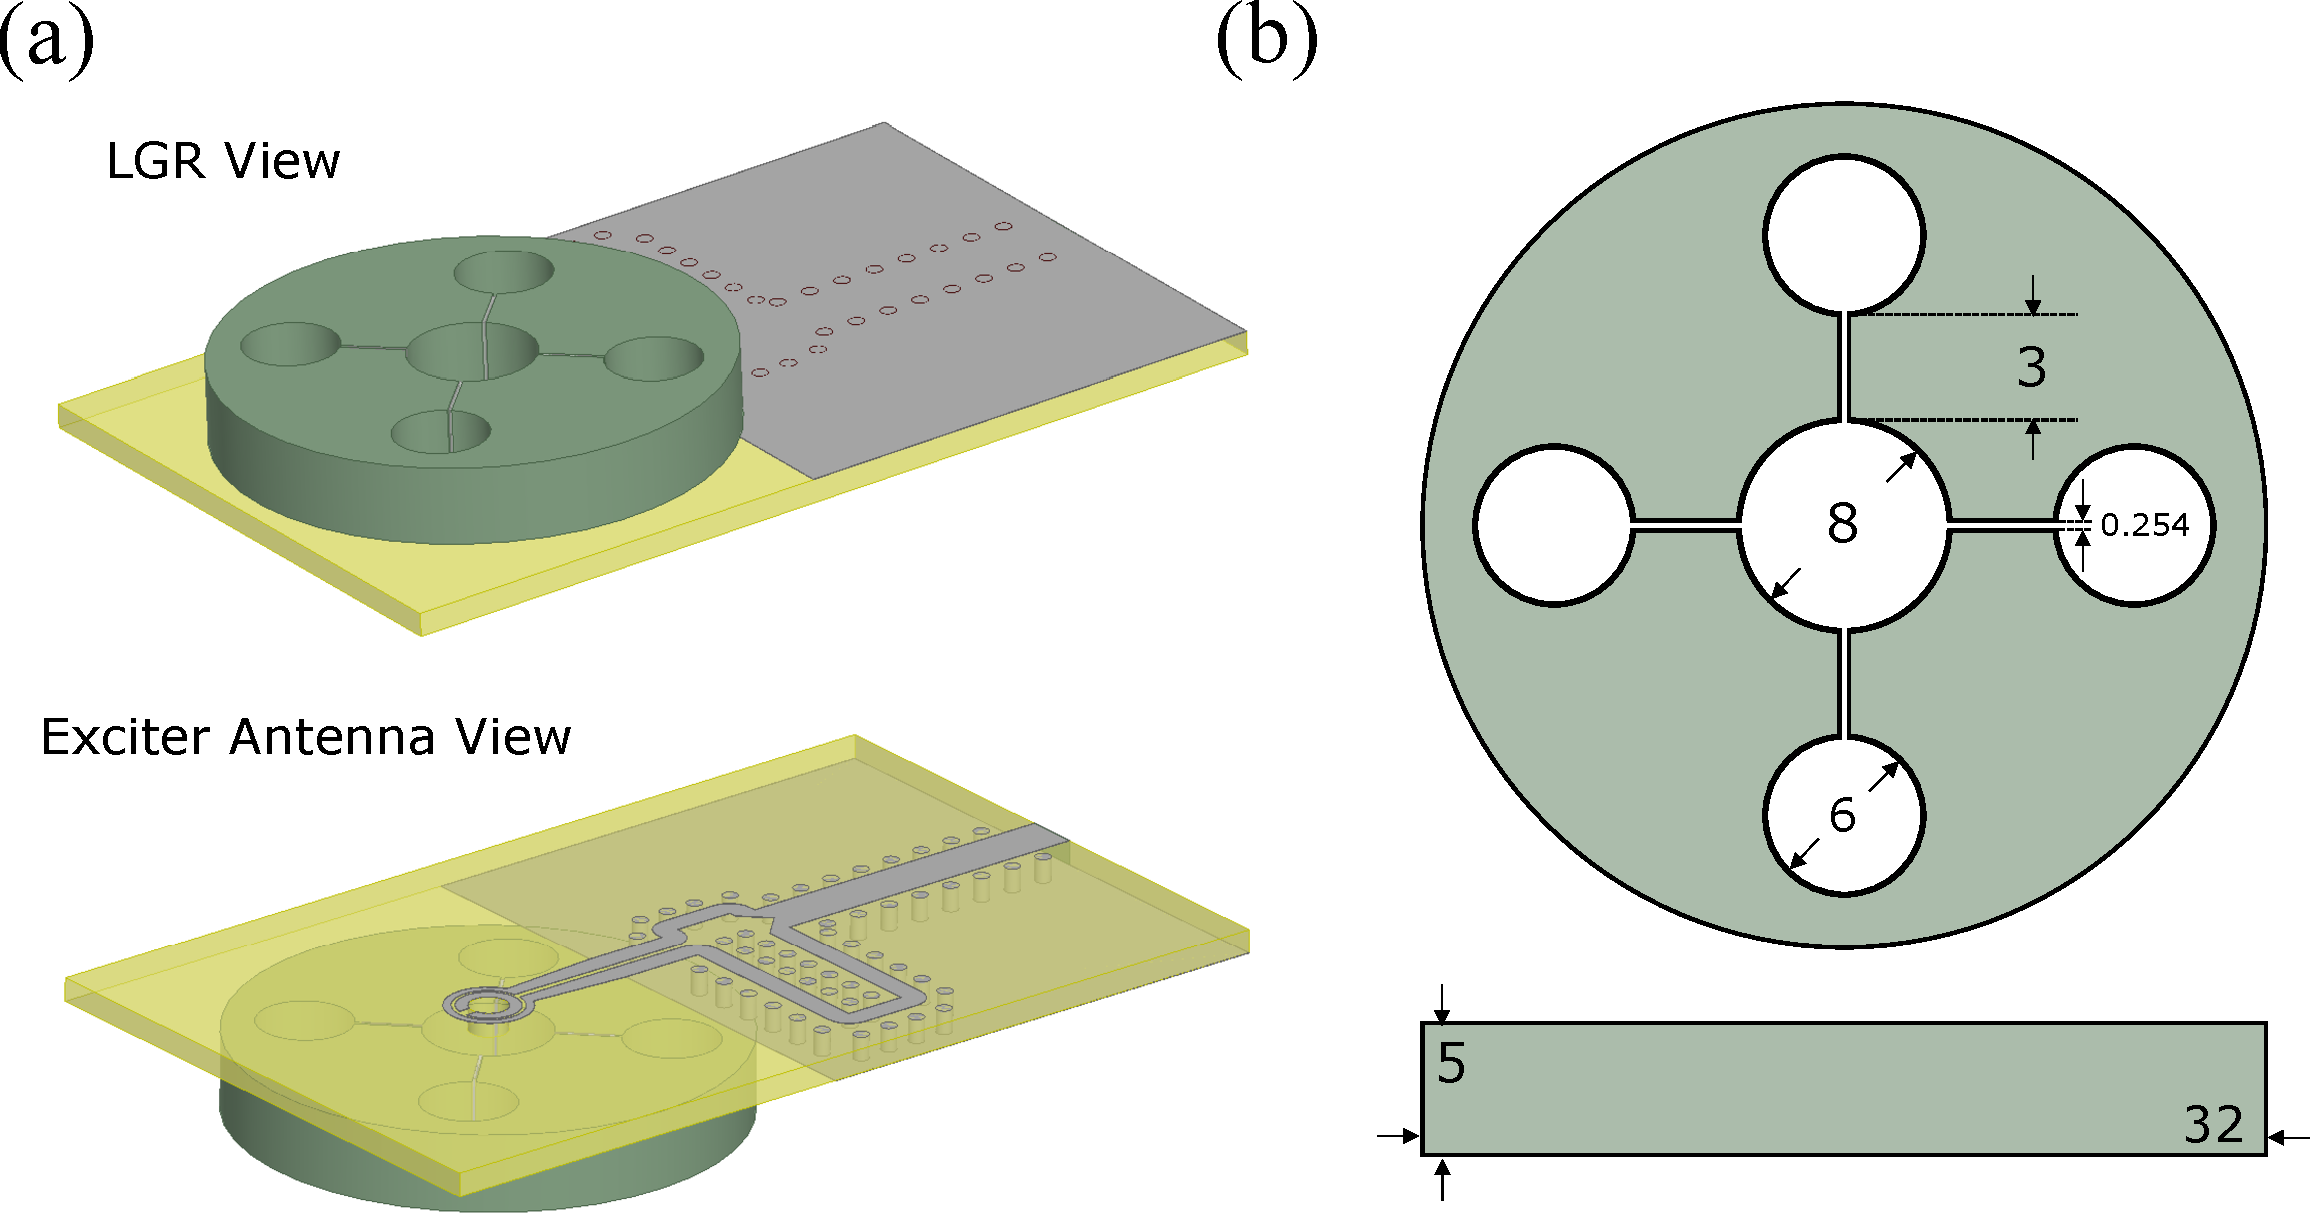
\includegraphics[width = \textwidth]{LGR_Image.pdf}  
\caption{\textbf{Rendering and Wire Diagram of Loop Gap Resonator} \textbf{a)} The metallic resonator employs a five-loop four-gap architecture. Microwaves are coupled into the LGR via the exciter antenna, which is fabricated on a printed circuit board. \textbf{b)} Line drawing of the LGR. All dimensions are in mm. Optional mounting holes and radial access port for laser excitation are now shown.}
\label{LGR_drawing}
\end{figure}

In practice, the central loop diameter is set to $\sim 5-10 $ mm, corresponding to the typical size of a diamond plate. The outer loop diameters are chosen to match the inner diameters within a small factor to ensure return flux is captured and does not extend into the annular region around the LGR \cite{}. Since the outer and inner loops set the effective inductance of the resonator, the gap area $A$ is constrained by the dual LGR design objectives of (i) maintaining optical accessibility, which limits the thickness of the device, and (ii) bounding $f_0$ above the target resonant frequency in order to allow for further tuning vie dielectric shims (discussed in section \ref{tuning}). Additionally, while increasing the number $n$ of loops and gaps can improve $B_1$ uniformity \cite{piasecki1993field} and lower the LGR's resonant frequency, this approach results in a denser mode spectrum \cite{froncisz1982loop} and increases the likelihood of cross-mode excitations deleteriously altering the field distribution within the central loop. As a compromise, the design employs $n=4$ outer loops [Fig. \ref{LGR_drawing} (a)] allowing for sufficient uniformity while locating the closest eigenmode more than 1.5 GHz below the TE\textsubscript{10} eigenmode [Fig \ref{}].  

The LGR in this work therefore consists of a central loop with radius $r_c = 4$ mm surrounded by four symmetrically arranged outer loops of radius $r_o = 3$ mm as shown in Figure \ref{LGR_drawing} (b). The outer loops return magnetic flux to the central loop and therefore oscillate antisymmetrically with the central loop ($\pi$ out of phase). The side walls of the capacitive gaps are separated by $d = 254$ $\upmu$m. With these dimensions, using equations \ref{induct} and \ref{cap}, $L = 8.7$ nH and $C = 0.17$ pF, resulting in an expected resonant frequency for the naked air-gapped LGR of $f_0 = 4.1$ GHz, approximately 1.2 GHz above the NV resonance frequencies.

An eigenfrequency simulation of the resonator using the geometrical parameters listed above was completed in ANSYS HFSS and the distribution of the magnetic flux density ($B_1$) for the TE\textsubscript{10} mode is depicted in Figure \ref{LGR_Eigen}. As mentioned above, for this mode the center loop oscillates $\pi$ radians out of phase with the outer loops. For the air-gapped resonator, HFSS returns a real eigenfrequency at 4.57 GHz (depicted in Figure \ref{LGR_Eigen} ) 

\begin{figure}[h!]
\centering
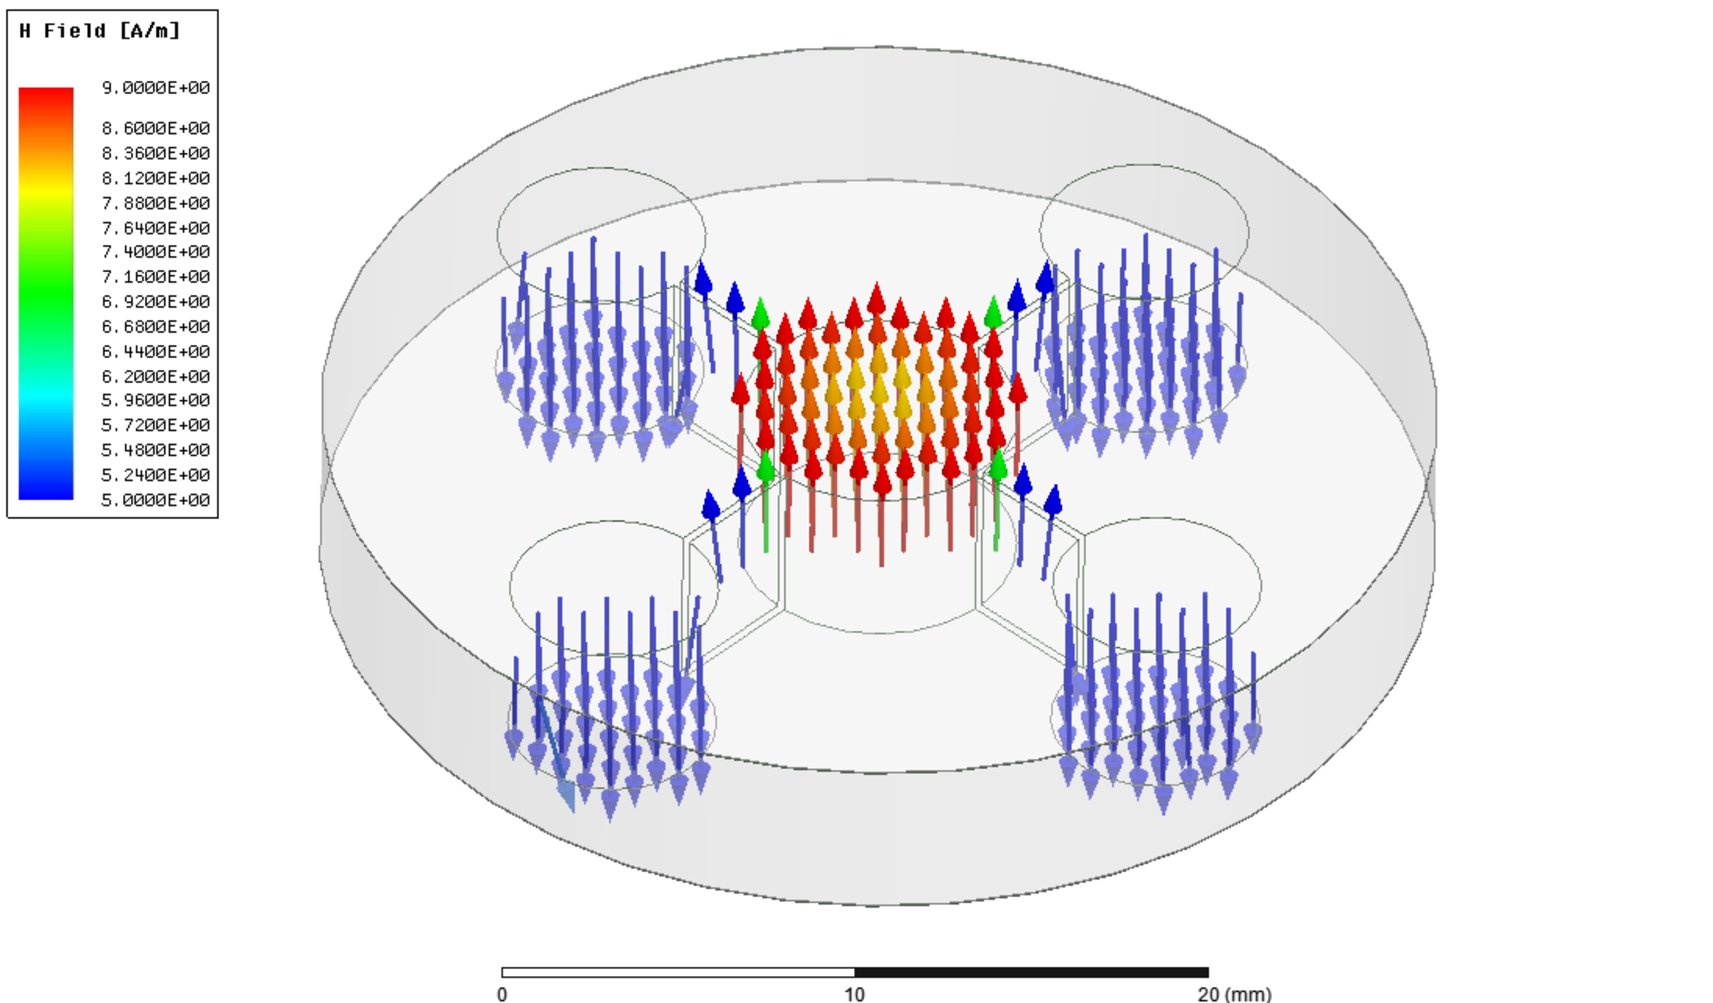
\includegraphics[width = \textwidth]{Eigen_Res.pdf}  
\caption{\textbf{Eigenfrequency solution to LGR} Eigenfrequency solution for TE\textsubscript{10} mode. The outer loops are oscillating $pi$ radians out of phase with center loop}
\label{LGR_Eigen}
\end{figure}


\section{Tuning} \label{tuning}

Talk about tuning the LGR using sapphire shims; why use sapphirie shims? etc etc etc

\section{Excitation Design}

To couple MW power into the LGR we utilized two separate methods, each to be used for different NV applications. For magnetic  microscopy, complete 2$\pi$ steradian optical access to the center cavity is of the utmost importance. For such modalities lateral coupling using a shorted coaxial loop [Figure \ref{} (a)] can be used to minimize the blocking of optical access to the central loop. Using this method, resonator coupling (described in section \ref{coupling}) is modified by changing the coaxial loop position in $z$ relative to the LGR. In this way the LGR can be quickly and effectively critically coupled for any shim configuration (ie. resonant frequency) [Figure \ref{} (b)].  



Discussion with images of coupling using shorted coax loop.

More robust coupling for implementable device

Discussion of split ring exciter antenna and design outline of feedline and balun and design process of stepping through circuit etc.

center loop coupling with split ring resonator. Sonnet program design or split loop (snap shots from program and S11 etc) 

\begin{figure}[t!]
\centering
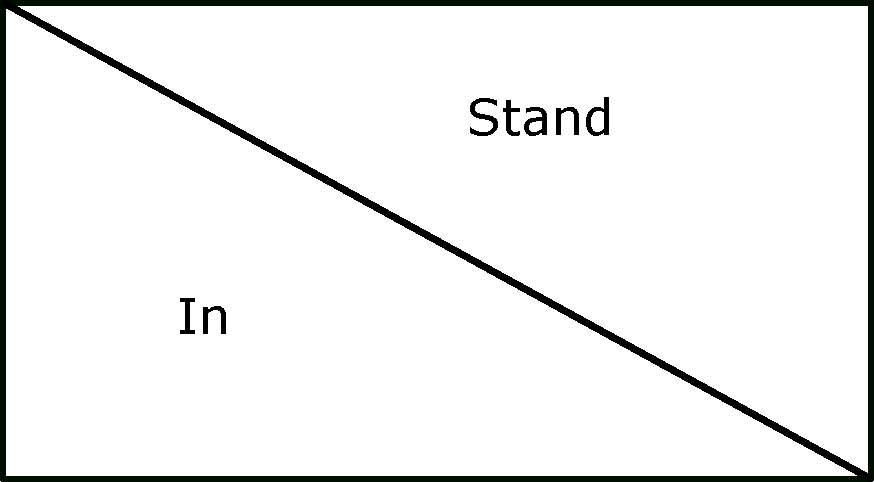
\includegraphics[width = \textwidth]{STANDIN.pdf}  
\caption{\textbf{Eigenfrequency solution to LGR} \textbf{a)} \textcolor{red} {STANDIN. PLEASE REPLACE}}
\label{LGR_Eigen}
\end{figure}


\section{Matching}

As mentioned above, for lateral coupling using a coaxial loop the LGR can be quickly matched to the feedline by varying the distance $z$ between the loop and the resonator. 






Talk about matching using coupling parameter and etc. (quick overview of matching using mathematical framework).

Talk about matching using Lateral loop coupling

Talk about Balun design (w/ sonnet)

Talk about board design (w/ sonnet)

Talk about additional matching using stub tuner.


\begin{figure}[h!]
\centering
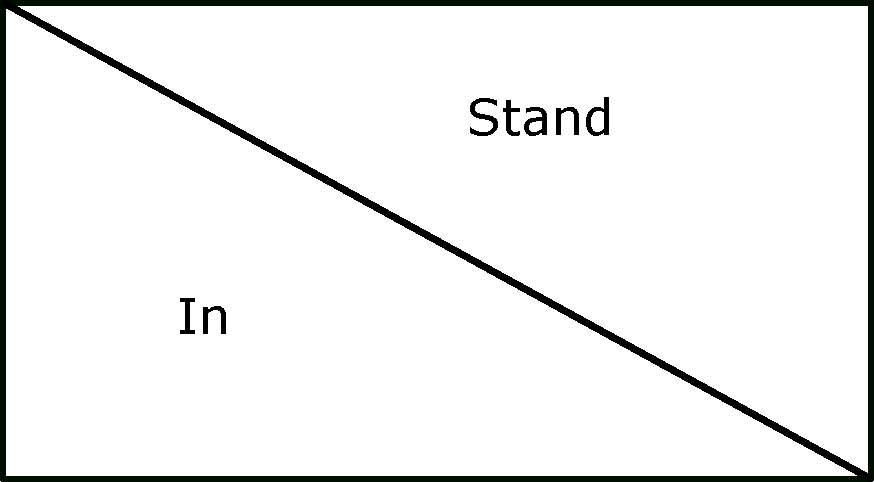
\includegraphics[width = \textwidth]{STANDIN.pdf}  
\caption{\textbf{Eigenfrequency solution to LGR} \textbf{a)} \textcolor{red} {STANDIN. PLEASE REPLACE}}
\label{LGR_Eigen}
\end{figure}



